\documentclass[11pt, english]{article}
%\usepackage[latin1]{inputenc}
\usepackage[T1]{fontenc}
\usepackage[utf8]{inputenc}
\usepackage[english]{babel}   % S P R A A K
% \usepackage{graphicx}    % postscript graphics
\usepackage{amssymb, amsmath, amsthm} % symboler, osv
\usepackage{mathrsfs}
\usepackage{url}
\usepackage{thmtools}
\usepackage{enumerate}  % lister $  
\usepackage{float}
\usepackage{tikz}
\usepackage{tikz-cd}
\usetikzlibrary{calc}
%\usepackage{tikz-3dplot}
\usepackage{subcaption}
\usepackage[all]{xy}   % for comm.diagram
\usepackage{wrapfig} % for float right
\usepackage{hyperref}
\usepackage{mystyle} % stilfilen      

%\usepackage[a5paper,margin=0.5in]{geometry}


\begin{document}
\title{Results}
\author{Fredrik Meyer}
\maketitle 

\section{Construction of a smooth Calabi-Yau}

Let $X_0$ be the Stanley-Reisner scheme corresponding to the join of two hexagons. Call this simplicial complex for $\mathcal K$. Then consider the join of $\K$ with $\Delta^1$. This corresponds to adding two free variables. The resulting Stanley-Reisner scheme $Y_0$ corresponds to a $5$-dimensional ball. 

By standard ``Sturmfels theory'', $Y_0$ deforms to a toric variety $Y$, whose associated polytope is the join of two hexagons. Since $X_0$ sits inside $Y_0$ as a linear section, it deforms as well to a generic hyperplane section in $Y$. $Y$ sits inside $\PP^{13}$, and its ideal sheaf is the sum of the ideal sheaf of two del Pezzo surfaces in $\PP^6$, anti-canonically embedded. It follows that the singular locus of $Y$ is $2$-dimensional, consisting of two disjoint copies of a del Pezzo surface. 

Hence the intersection of $Y$ with two generic hyperplanes is a 3-dimensional variety with isolated singularities. Since the del Pezzos are of degree $6$, there should in total be $12$ singularities, looking locally like cones over del Pezzos. In the following we will try to describe their topology.

There exists a deformation of $Y$, reducing its singular locus to a normal crossing cycle of dimension $1$. This implies that there exists a smoothing of $X_0$, yielding a smooth Calabi-Yau. One of our main tasks will be to try to compute some of its invariants.

\subsection{Recipe for finding the smoothing}

This is a general heuristic for finding smoothings of Stanley-Reisner schemes, which worked well in my master's thesis, where I studied degenerations of the Grassmannian $\Gr(3,6)$.

The main ingredient will be the package \texttt{Macaulay2} package \texttt{VersalDeformations} by Nathan Ilten. It comes with a method that takes as input an ideal, a basis for the first-order deformations, and a basis for the obstruction space. Then the algorithm tries to successively lift the equations to higher order. One can optionally only give the algorithm a subset of a basis of the first-order deformations. 

[[rediscover this]]

\subsection{Dimension of some cohomology groups}

\begin{tabular}{ l || c | r | r | r | r | r | c  }
 Group & 0 & 1 & 2 & 3 & 4 & 5 & Euler-characteristic \\
\hline
$H^i(X, \Omega_{\PP^{12}} \otimes \OO_X)$ & 0 & 1 & 0 & 167 & 0 & 0 & -168\\
$H^i(Y, I_Y/I_Y^2)$ & 0 & 36 & 0 & 12 & 2 & 0 & -46 \\
$H^i(Y, \Omega_Y)$ & 0 & 1  & 12 & 2 & 0  & 0 & -9
\end{tabular}


\section{The singular locus of $Y$}

By computing in each chart and taking closures, it can be computed that the singular locus of $Y$ is of dimension $1$, and consists of the union of 
projective lines. [[do this explcitily]]

\section{Descriptions of $dP_6$}

Recall that $dP_6$ is the toric variety whose associated polytope is the hexagon:
 
\begin{center}
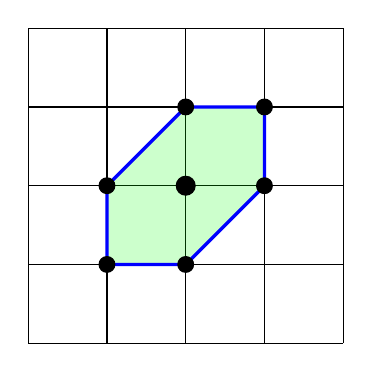
\begin{tikzpicture}
  \draw (0, 0) grid (4, 4);  

\draw [very thick, color=blue, fill=green, fill opacity=0.2]
(1,1) -- (2,1) -- (3,2) -- (3,3) -- (2,3) -- (1,2) -- cycle;

\draw [fill=black]  (1, 1) circle (0.1);
\draw [fill=black]  (2, 1) circle (0.1);
\draw [fill=black]  (3, 2) circle (0.1);
\draw [fill=black]  (3, 3) circle (0.1);
\draw [fill=black]  (2, 3) circle (0.1);
\draw [fill=black]  (1, 2) circle (0.1);
\draw [fill=black]  (2, 2) circle (0.12);
\end{tikzpicture}
\end{center}


This induces an embedding into $\PP^6$, by standard toric geometry. Let $\PP^6$ have coordinates $y_0,x_1..x_6$ (corresponding to the center and the vertices, respectively). Then the ideal of $dP_6$ inside $\PP^6$ is given by the $2 \times 2$-minors of the matrix
\begin{equation}
\label{eqdp6}
\begin{vmatrix}
x_1 & y_0 & x_6 \\
x_2 & x_3 & y_0 \\
y_0 & x_4 & x_5
\end{vmatrix} \leq 1.
\end{equation}

The $\Z_6$-symmetry is visible by permuting columns and rows. 

Note that this representation of the ideal gives us an embedding of $dP_6$ into $\PP^2 \times \PP^2$ as a section of $\OO_{\PP^2 \times \PP^2}(1,1)\oplus\OO_{\PP^2 \times \PP^2}(1,1)$ (namely as the zeros of $t_{12}-t_{23}=t_{23}-t_{31}$ (where $t_{ij}$ are the natural coordinates on the product).

There are several other ways to veiw $dP_6$.

\subsection{As $\PP^2$ blown up in 3 points}

Consider the monoidal transformation $\varphi:\PP^2 \to \PP^2$ given by $(u:v:w) \mapsto (uv:uw:vw)$. This is a birational involution with three points of indeterminacy: $P_1=(1:0:0)$, $P_2=(0:1:0)$ and $P_3=(0:0:1)$. We blow up $\PP^2$ in these three points to get a scheme $\widetilde X$ and a morphism $\pi:\widetilde X \to \PP^2$. Then $dP_6$ is $\widetilde X$.

\begin{remark}
Note that the involution $\widetilde \varphi $ lifts to an involution  $\widetilde \varphi: \widetilde X \to \widetilde X$. We can realize $\widetilde X$ as the closure of the graph of $\varphi$:
$$
\widetilde X = \{ (u:v:w) \times  (a:b:c) \in \PP^2 \times \PP^2 \mid vb=wa=uc \}.
$$
Then the involution is $\widetilde \varphi(u:v:w,a:b:c) = (a:b:c, u:v:w)$.
\end{remark}

It can be shown that the automorphism group of $dP_6$ is $(\C^\ast)^2 \rtimes (S_2 \times S_3)$ ([DOLGACHEV]). The lifted involution $\widetilde \varphi$ generates the $S_2$ part. The $(\C^\ast)^2$-part is inherited from the corresponding action on $\PP^2$ and it can be computed to be given by
$$
(t_1,t_2) \cdot ((u:v:w)\times (a:b:c)) = (t_1u,t_2v, t_1^{-1}t_2^{-1}w) \times (t_1t_2a: t_2^{-1}b: t_1^{-1} c).
$$

The $S_3$ part comes from permuting the three points $P_1$, $P_2$ and $P_3$. If $\sigma \in S_3$ is a permutation of the variables $u,v,w$, then the corresponding action on $\widetilde X$ is given by $\sigma (P \times Q)=\sigma P \times \sigma^{-1} Q$. For example, the cyclic part is generated by
$$
(u:v:w)\times (a:b:c) \mapsto (w:u:v) \times(b:c:a).
$$


\subsection{A natural embedding in $\PP^1 \times \PP^1 \times \PP^1$}

Let $D$ be the divisor $D=2(u)+2(v)+2(w)$ in $Div(\PP^2)$ and consider the linear system $\lvert D \rvert$. Let 
\begin{align*}
 f_1 = \frac{uv}{w^2} && f_2 = \frac{uw}{v^2} && f_3 = \frac{vw}{u^2}
\end{align*}
be three sections. Together they define a rational map $\PP^2 \rmap \PP^1 \times \PP^1 \times \PP^1$. The base locus consist exactly of the three points $P_1,P_2,P_3$ above. So again we can blow up to resolve the locus of indeterminacy to get a map $\widetilde X \to {(\PP^1)}^3$.

If $t_i,s_i$ are coordinates on $\PP^1 \times \PP^1 \times \PP^1$ for $i=1,2,3$, then the equation of the image is given by $t_1t_2t_3=s_1s_2s_3$. 

\section{Deformations of $dP_6$}

Since $dP_6$ is smooth, the only singularity of its affine cone, $C(dP_6)$, is the origin. One can compute that $T^1(C(dP_6))=3$, and that the versal base space splits into two components: a line and a plane intersecting transversely.

\subsection{The first smoothing of the affine cone}

We attempt to give explicit descriptions of the two affine smoothing components of $C(dP_6)$. 

One of the components is given by:
\[
\begin{vmatrix}
x_1 & y_0 & x_6 \\
x_2 & x_3 & y_0-t_1 \\
y_0-t_2 & x_4 & x_5
\end{vmatrix} \leq 1.
\]

That is, as the $2 \times 2$-minors of the above matrix. This time we see that the affine cone $C(dP_6)$ embeds naturally in the affine cone over $C(\PP^2 \times \PP^2)$, again as the intersection of two hyperplanes, but with some coefficients added.

It can be computed that the locus of points in $\Aa^2$ with singular fibers have ideal generated by $st(s+t)=s^2t+t^2s$, namely the union of the axes and a line.

\subsection{The other smoothing of the affine cone}

The other smoothing is derived from another way of writing the equations of $dP_6$. See Figure 1. One obtains the equations for this ``$2 \times 2 \times 2$-tensor'' by taking $2 \times 2$-minors along the faces and along long diagonals.


\begin{figure}
\centering 
  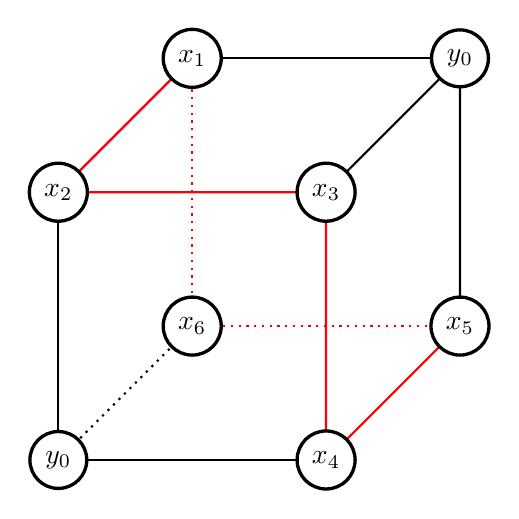
\begin{tikzpicture}[scale=1.7,every node/.style={circle, draw=black, fill=white}, every path/.style={very thick}]
\coordinate (A) at (0,0);
\coordinate (B) at (2,0);
\coordinate (C) at (2,2);	
\coordinate (D) at (0,2);	
\coordinate (E) at (1,1);	
\coordinate (F) at (3,1);	
\coordinate (G) at (3,3);	
\coordinate (H) at (1,3);	

\draw[thick, color=red] (D)  -- (C) -- (B) --(F);  %1
\draw[thick, color=red, dotted] (H) -- (E);
\draw[thick, color=red, dotted] (E) -- (F);
\draw[thick, color=red] (D) -- (H);
\draw[thick] (D) -- (A) -- (B);
\draw[thick] (C) -- (G) -- (F);
\draw[thick] (H) -- (G);
\draw[thick, dotted] (A) -- (E);

\draw (A) node {$y_0$};
\draw (B) node {$x_4$};
\draw (C) node {$x_3$};
\draw (D) node {$x_2$};
\draw (E) node {$x_6$};
\draw (F) node {$x_5$};
\draw (G) node {$y_0$};
\draw (H) node {$x_1$};
\end{tikzpicture}
  \caption{Equations of $\PP^1 \times \PP^1 \times \PP^1$.}
\end{figure}

\begin{figure}
\centering 
  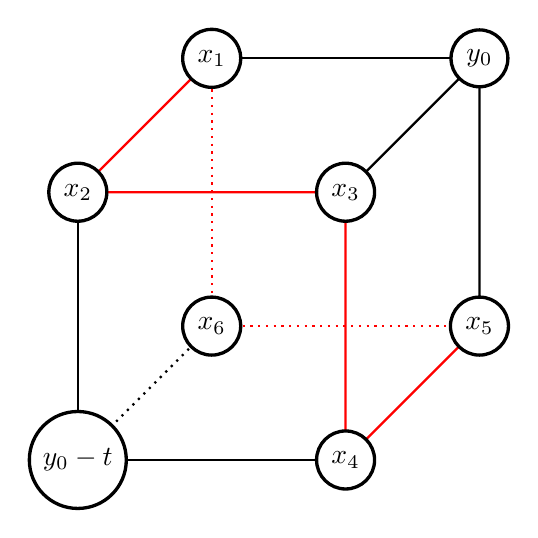
\begin{tikzpicture}[scale=1.7,every node/.style={circle, draw=black, fill=white}, every path/.style={very thick}]
\coordinate (A) at (0,0);
\coordinate (B) at (2,0);
\coordinate (C) at (2,2);	
\coordinate (D) at (0,2);	
\coordinate (E) at (1,1);	
\coordinate (F) at (3,1);	
\coordinate (G) at (3,3);	
\coordinate (H) at (1,3);	

\draw[thick, color=red] (D)  -- (C) -- (B) --(F);  %1
\draw[thick, color=red, dotted] (H) -- (E);
\draw[thick, color=red, dotted] (E) -- (F);
\draw[thick, color=red] (D) -- (H);
\draw[thick] (D) -- (A) -- (B);
\draw[thick] (C) -- (G) -- (F);
\draw[thick] (H) -- (G);
\draw[thick, dotted] (A) -- (E);

\draw (A) node {$y_0-t$};
\draw (B) node {$x_4$};
\draw (C) node {$x_3$};
\draw (D) node {$x_2$};
\draw (E) node {$x_6$};
\draw (F) node {$x_5$};
\draw (G) node {$y_0$};
\draw (H) node {$x_1$};
\end{tikzpicture}
  \caption{Deforming $C(dP_6)$.}
\end{figure}

It is clear that the one-dimensional component is a smoothing of $C(dP_6)$, since it can be obtained as a generic hyperplane in $C(\PP^1 \times \PP^1 \times \PP^1)$.

\section{Topology of the smootings of the affine cones}

Since the singularities of our Calabi-Yau look locally like affine cones over $dP_6$, and the smoothings are given by locally smoothing these cones, we would like to compute their topology. 

\subsection{The first smoothing of $C(dP_6)$}

Recall that one of the smoothing components of $C(dP_6)$ is given by the equations of $\PP^1 \times \PP^1 \times \PP^1$ in its Segre embedding in $\PP^7$, replacing one of the corners by $y_0+t$.

The total family lies in $\Aa^8$, and we can take its projective closure in $\PP^8$ by homogenizing the equations (treating the variable $s_1$ as a constant of degree $0$). Thus we get a family $\mathscr X \to \Aa^1$, where $\mathscr X_s$ is a projective variety for each $s \in \Aa^1$. For $s=0$, we get the projective cone over $dP_6$, and for $s \neq 0$, we get something isomorphic (after a linear change of coordinates) to $(\PP^1)^3$. By inspection, we see that what is gained in the projective closure is exactly $dP_6$ (for $s \neq 0$). Hence the smoothing of $C(dP_6)$ is isomorphic to $\PP^1 \times \PP^1 \times \PP^1 \bs dP_6$.

Let $M = \PP^1 \times \PP^1 \times \PP^1$ and let $D=dP_6$. There is the so-called ``homology Gysin sequence'' (from \cite{dimca_singularities}), which will help us compute much of the homology of $M$:

\[
\ldots \to H_{k+1}(M) \to H_{k-1}(D) \to H_k(M \bs D) \to H_k(M) \to H_{k-2}(D) \to H_{k-1}(M \bs D) \to \ldots 
\]

Since $\PP^1 \simeq S^2$, we can use the Künneth formula to compute the homology of $(\PP^1)^3$: 
\[
H^i(M) = \begin{cases}
1 & i = 0 \\
0 & i = 1 \\
3 & i = 2 \\
0 & i = 3 \\
3 & i = 4 \\
0 & i = 5 \\
1 & i = 6
\end{cases}
\]

The homology of the del Pezzo is given by 

\[
H^i(D) = \begin{cases}
1 & i = 0 \\
0 & i = 1 \\
4 & i = 2 \\
0 & i = 3 \\
1 & i = 4
\end{cases}
\]

Writing up the long exact sequence (and being happy for all the zeroes), we find almost all the homology of $M \bs D$: (NOT TRUE)
\[
H^i(M \bs D) = \begin{cases}
1 & i = 0 \\
0 & i = 1 \\
2 & i = 2 \\
? & i = 3 \\
?' & i = 4 \\
0 & i = 5,6.
\end{cases}
\]

The two questions marks are not independent, however. Since $\chi(M) = 8$\footnote{Heuristic: Euler-characteristic is some kind of volume. And $\PP^1$ has Euler characteristic two, and volume should be multiplicative.} and $\chi(dP_6)=6$, we know that $\chi(M \bs D) = 2$. In fact, $?'=?-1$. ((there may be some codimension argument to the effect that $H_4(M) = H_4(M \bs D)$ ...))

\subsubsection{Lefschetz duality}

We have the following theorem from \cite[Chapter 6, p.~297]{spanier_topology}. Let $R$ be a ring.

\begin{thm}[Lefschetz duality]
Let $(M,D)$ be a compact relative $n$-manifold such that $M\bs D$ is orientable over $R$. For all $q$ and $R$-modules $M$, there is an isomorphism
$$
H_q(M \bs D ) \simeq \overline H^{n-q}(M,D;G).
$$
\end{thm}

We can use this to find the cohomology of the complement $M \bs D$, provided we are able to do some explicit calculations. Namely, the long exact sequence of a pair gives us (let $M=\PP^1 \times \PP^1 \times \PP^1$ and let $D=dP_6$)
$$
0 \to H^4(M,D) \to H^4(M) \xrightarrow{j^\ast} H^4(D) \to H^5(M,D) \to 0.
$$
The map $j^\ast$ is the map on cohomology induced from the inclusion $D \hookrightarrow M$. The last term is equal to $H_1(M \bs D)$ by Lefschetz duality. Hence it is either $1$- or $0$-dimensional (up to torsion). 

Hence we would like to compute the map $j^\ast: H^4(M) \to H^4(V)$ explicitly.

\subsection{The second smoothing}

\begin{prop}
The second smoothing $M_2$ is isomorphic to $(\PP^2 \times \PP^2) \cap H \bs dP_6$, where $H$ is a hyperplane section.
\end{prop}
\begin{proof}
Compare the equations of the Segre embedding of $\PP^2 \times \PP^2$ with the equations of a generic fiber of the second smoothing:
\begin{align*}
\begin{vmatrix}
x_1 & y_0 & x_6 \\
x_2 & x_3 & y_0+t \\
y_0+s & x_4 & x_5
\end{vmatrix} \le 1
&&
\begin{vmatrix}
x_1 & y_0 & x_6 \\
x_2 & x_3 & y_1 \\
y_2 & x_4 & x_5
\end{vmatrix} \le 1.
\end{align*}
Homogenize the first equations with respect to the variable $y_1$. Then, in the coordinates of $\PP^8$, the homogenized variety corresponds to the variety given as $(\PP^2 \times \PP^2) \cap \{ (t(t_{32}-t_{11})=s(t_{23}-t_{11}) \}$.

Now we check what we gained by homogenizing. $\PP^8 \bs \Aa^8$ is given by the divisor $\{ y_1 = 0 \}$, but this is exactly equal to $dP_6$.
\end{proof}

We can use this, and the homological Gysin sequence to compute some of the cohomology of $M_2$




\bibliographystyle{plain}
\bibliography{bibliografi}

\end{document}
